\chapter{Circuiti combinatori e algebra di Boole}

\section{Algebra di Boole}\label{sec:algebra_di_boole}
Partiamo dall'algebra perchè vogliamo costruire circuiti più efficienti possibili. In particolar modo all'algebra di commutazione perchè fa riferimento ai procedimenti dei calcolatori.

L'algebra di Boole è fomata da:
\begin{itemize}
    \item Un alfabeto di supporto. $\Sigma = \{0,1\}$;
    \item Da operazioni booleane quali:
    \begin{itemize}
        \item \textbf{Not}. Dato $a$, not $a=\overline{a}$\\
            \begin{figure}[htp]
                \centering
                \hfill
                \begin{minipage}[b]{.3\columnwidth}
                    \centering
                    \begin{tabular}{c|c}
                         $a$ & $\overline{a}$\\\hline
                         0 & 1\\
                         1 & 0
                    \end{tabular}
                    \caption{Tabella di verità del not}\label{tab:not}
                \end{minipage}\hfill
                \begin{minipage}[b]{.3\columnwidth}
                    \centering
                    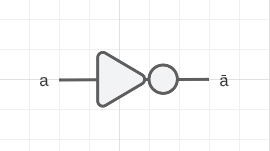
\includegraphics[width = 5cm]{images/porta_not.JPG}
                    \caption{Porta logica del not}\label{fig:boole_not}
                \end{minipage}\hspace*{\fill}
            \end{figure}
        \item \textbf{And}. Dati $a$ e $b$, and $=a*b$\\
            \begin{figure}[htp]
                \centering
                \hfill
                \begin{minipage}[b]{.3\columnwidth}
                    \centering
                    \begin{tabular}{c|c}
                         $a,b$ & $a*b$\\\hline
                         00 & 0\\
                         01 & 0\\
                         10 & 0\\
                         11 & 1
                    \end{tabular}
                    \caption{Tabella di verità dell'and}\label{tab:and}
                \end{minipage}\hfill
                \begin{minipage}[b]{.3\columnwidth}
                    \centering
                    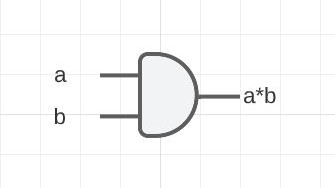
\includegraphics[width = 5cm]{images/porta_and.JPG}
                    \caption{Porta logica dell'and}\label{fig:boole_and}
                \end{minipage}\hspace*{\fill}
            \end{figure}
        \item \textbf{Or}. Dati $a$ e $b$, or $=a+b$\\
            \begin{figure}[htp]
                \centering
                \hfill
                \begin{minipage}[b]{.3\columnwidth}
                    \centering
                    \begin{tabular}{c|c}
                         $a,b$ & $a+b$\\\hline
                         00 & 0\\
                         01 & 1\\
                         10 & 1\\
                         11 & 1
                    \end{tabular}
                    \caption{Tabella di verità dell'or}\label{tab:or}
                \end{minipage}\hfill
                \begin{minipage}[b]{.3\columnwidth}
                    \centering
                    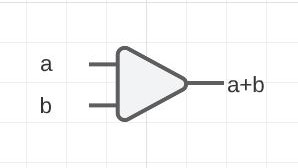
\includegraphics[width = 5cm]{images/porta_or.JPG}
                    \caption{Porta logica dell'or}\label{fig:boole_or}
                \end{minipage}\hspace*{\fill}
            \end{figure}
    \end{itemize}
\end{itemize}



\subsection{Assiomi e proprietà}
L’algebra booleana si basa su un insieme di postulati che come tali vengono per definizione considerati corretti. I postulati non sono dimostrabili, nel senso che un assunto di partenza non può essere dimostrato. A partire da questi postulati è possibile invece dimostrare tutti i teoremi dell’algebra booleana.

Le proprietà e gli assiomi dell’algebra booleana obbediscono al principio di \textbf{dualità}: se i simboli 0 e 1 e gli operatori $*$ (AND) e $+$ (OR) sono scambiati tra loro, l’affermazione rimane corretta.

\subsubsection*{Assiomi}
\begin{definition}[Associatività]
    \begin{equation}
        a+(b+c)=(a+b)+c
    \end{equation}
    \begin{equation*}
        a(b*c)=(a*b)c
    \end{equation*}
\end{definition}

\begin{definition}[Commutatività]
    \begin{equation}
        a+b=b+a
    \end{equation}
    \begin{equation*}
        a*b=b*a
    \end{equation*}
\end{definition}

\begin{definition}[Distributività]
    \begin{equation}
        a(b+c)=a*b+a*c
    \end{equation}
    \begin{equation*}
        a+b*c=(a+b)(a+c)
    \end{equation*}
\end{definition}

\begin{definition}[Elemento neutro]
    \begin{equation}
        a+0=a
    \end{equation}
    \begin{equation*}
        a*1=a
    \end{equation*}
\end{definition}

\begin{definition}[Complemento]
    \begin{equation}
        a+\overline{a}=1
    \end{equation}
    \begin{equation*}
        a*\overline{a}=0
    \end{equation*}
\end{definition}

\subsubsection*{Proprietà}
\begin{definition}[Involuzione]
    \begin{equation}
        \overline{\overline{a}}=a
    \end{equation}
\end{definition}

\begin{definition}[Idempotenza]
    \begin{equation}
        a+a=a
    \end{equation}
    \begin{equation*}
        a*a=a
    \end{equation*}
\end{definition}

\begin{definition}[Elemento nullo]
    \begin{equation}
        a+1=1
    \end{equation}
    \begin{equation*}
        a*0=0
    \end{equation*}
\end{definition}

\begin{definition}[Assorbimento 1]
    \begin{equation}
        a+ab=a
    \end{equation}
    \begin{equation*}
        a(a+b)=a
    \end{equation*}
\end{definition}

\begin{definition}[Assorbimento 2]
    \begin{equation}
        a+\overline{a}b=a+b
    \end{equation}
    \begin{equation*}
        a(\overline{a}+b)=ab
    \end{equation*}
\end{definition}

\begin{definition}[Leggi di Morgan]
    \begin{equation}
        \overline{a+b}=\overline{a}*\overline{b}
    \end{equation}
    \begin{equation*}
        \overline{a*b}=\overline{a}+\overline{b}
    \end{equation*}
\end{definition}

\begin{description}
    \item[N.B.] Assiomi e proprietà valgono anche per le espressioni booleane.
\end{description}

\section{Espressioni booleane}
\begin{itemize}
    \item Un letterale è un'espressione booleana così come lo sono 0 e 1;
    \item Se $E$ è un'espressione booleana, allora $\overline{E}$ è un'espressione booleana;
    \item Se $E_1$ e $E_2$ sono espressioni booleane, anche $E_1+E_2$ ed $E_1*E_2$ sono espressioni booleane;
    \item Sono espressioni booleane tutte e sole quelle che otteniamo con le espressioni precendenti.
\end{itemize}

\subsection{Trasformazione o semplificazione di espressioni booleane}
\begin{exercise}
    $a+b(\overline{c+d\overline{a}})$\\
    \begin{center}
    \begin{tabular}{c r}
        Espressione & Proprietà\\\hline\\
         $a+b(\overline{c}(\overline{d\overline{a}}))$ & De Morgan\\
         $a+b(\overline{c}(\overline{d}+\not\overline{\overline{a}})$ & De Morgan + involuzione\\
         $a+b(\overline{c}\overline{d}+\overline{a}\overline{c})$ & Distributiva\\
         $a+b\overline{c}\overline{d}+ab\overline{c}$ & Distributiva\\
         $a(1+b\overline{c})+b\overline{c}\overline{d}$ & Raggruppo + elemento nullo\\
         $a+b\overline{c}\overline{d}$ & Risultato
    \end{tabular}
    \end{center}
\end{exercise}

\subsection*{Verifica di identità}
\begin{exercise}\label{es:verifica_identita}
    $ab+bc+\overline{a}c=ab+\overline{a}c$
    \begin{center}
    \begin{tabular}{c r}
        Espressione & Proprietà\\\hline\\
        $ab+(a+\overline{a})bc+\overline{a}c$ & Moltiplico per 1, $a+\overline{a}$\\
        $ab+abc+\overline{a}bc+\overline{a}c$ & Assorbimento\\
        $ab+\overline{a}c$ & Risultato
    \end{tabular}
    \end{center}
\end{exercise}
Se un'identità è vera, anche la sua duale è vera. Quindi:
\begin{center}
    $(a+b)(b+c)(\overline{a}+c)=(a+b)(\overline{a}+c)$
\end{center}

\subsection{Espressione complementare}
L'espressione complemetare è un'identità che si ottiene negando l'espressione di partenza. Data $E$ la sua complementare è $\overline{E}$.
\begin{center}
    $E=ab+\overline{a}c\hspace{0,5cm}\overline{E}=\overline{ab+\overline{a}c}$
\end{center}
Per risolverla: $\overline{ab}+\overline{\overline{a}c}=(\overline{a}+\overline{b})(a+\overline{c})$

Riguradando l'esercizio \ref{es:verifica_identita} notiamo come i due risultati sono complementari.
Quindi per ottenere la complementare di un'espressione booleana, posso applicare de Morgan come nell'esempio oppure passare alla duale e complementare i singoli letterali.

\subsection*{Quanto vale un'espressione booleana?}
Il valore di un'espressione booleana si può ottenere tramite la tavola di verità.
\begin{exercise}\label{es:tavola_di_verita}
    $(a+b)(\overline{a}+c)$
    
    Quest'espressione si può risolvere lasciandola così ovvero come prodotto di somme (POS) oppure calcolando la duale e quindi come somma di prodotti (SOP).
    In entrambe i casi la tavola di verità è la seguente:
    \begin{table}[ht]
        \centering
        \begin{tabular}{|c|c|}
            \hline abc & f\\\hline\hline
            000 & 0\\\hline
            001 & 0\\\hline
            010 & 1\\\hline
            011 & 1\\\hline
            100 & 0\\\hline
            101 & 1\\\hline
            110 & 0\\\hline
            111 & 1\\\hline
        \end{tabular}
        \caption{Tavola di verità dell'esercizio \ref{es:tavola_di_verita}}
        \label{tab:my_label}
    \end{table}
\end{exercise}

\subsection{Espressioni in forma normale SOP/POS}
Per trasfomare espressioni booleane in forma normale SOP\footnote{Sum Of Products, Somma di prodotti}/POS\footnote{{Products Of Sum, Prodotto di somme}}, procediamo nel seguente ordine:
\begin{enumerate}
    \item Applicare de Morgan;
    \item Applicare la proprietà distributiva:
    \begin{itemize}
        \item SOP, $a(b+c)=ab+ac$;
        \item POS, $a+bc=(a+b)(a+c)$.
    \end{itemize}
    \item Eliminare termini rindondanti.
\end{enumerate}

\begin{example}
    $\overline{\overline{x_1}+x_2}+\overline{x_1}+x_3$\hspace{1cm}Forma SOP: $\overline{\overline{x_1}}\overline{x_2}+\overline{x_1}x_3$\hspace{1cm}$(x_1\overline{x_2}+\overline{x_1})(x_1\overline{x_2}+x_3)$\hspace{1cm}$(x_1+\overline{x_1})(\overline{x_2}+\overline{x_1})(x_1+x_3)(\overline{x_2}+x_3)$\hspace{1cm}Forma POS: $1(\overline{x_1}+\overline{x_2})(x_1+x_3)(\overline{x_2}+x_3)$
\end{example}

\subsection{Canonica SOP/POS}
Viene chiamata forma canonica l'espressione booleana dove tutti i fattori contengono tutti i letterati.
\begin{itemize}
    \item SOP se tutti prodotti sono mintermini\footnote{Ogni prodotto contiene tutti i letterali.};
    \item POS se tutte le somme sono maxtermini\footnote{Ogni somma contiene tutti i letterali.}.
\end{itemize}

Per ottenere la forma canonica da una forma normale si moltiplica per $x+\overline{x}$ nel caso della SOP, si somma per il prodotto $x\overline{x}$ nella POS, dove $x$ rappresenta l'elemento mancante. In tutti e due i casi infine si applica la proprietà distributiva e si eliminano i termini rindondanti.

\begin{description}
    \item[N.B.] Le forme canoniche permettono di stendere le tavole di verità con più facilità.
\end{description}

\begin{example}[SOP]
    Normale SOP: $a\overline{b}+\overline{a}c$\\La trasformo in forma canonica SOP:
    $\overline{ab}(c+\overline{c})+\overline{a}c(b+\overline{b})$\\ $a\overline{b}c+a\overline{b}\overline{c}+\overline{a}bc+\overline{a}\overline{b}c$
    
    Inserisco i valori ottenuti all'interno della tabella di verità.
    
    \begin{figure}[!htbp]
        \centering
        \hfill
        \begin{minipage}[b]{.3\columnwidth}
            \centering
            \begin{tabular}{c|c}
                 $a,b,c$ & $g$\\\hline
                 000 & 0\\
                 001 & 1\\
                 010 & 0\\
                 011 & 1\\\hline
                 100 & 1\\
                 101 & 1\\
                 110 & 0\\
                 111 & 0
            \end{tabular}
        \end{minipage}\hfill
        \begin{minipage}[b]{.3\columnwidth}
            \centering
            Identifico il prodotto delle equazioni con 1 nel letterale e 0 nella forma complementata.
            
            Es. $a\overline{b}c$ vale $a=1, \overline{b}=0, c=1$ e inserisco 1 nella tabella in corrispondenza del valore $101$.
        \end{minipage}\hspace*{\fill}
    \end{figure}
    
    Questo perchè il nosto obiettivo è quello di trovare i valori per cui il prodotto sia uguale a 1 (ovvero quando tutti i termini valgono 1).
    
    \begin{figure}[!htbp]
        \centering
        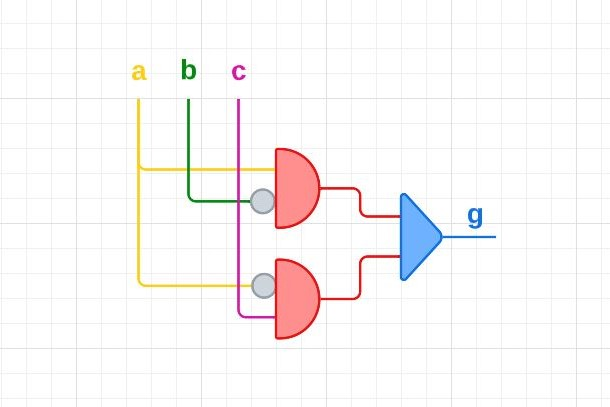
\includegraphics[width= 6cm]{images/cir_sop_fnor.JPG}\hfil
        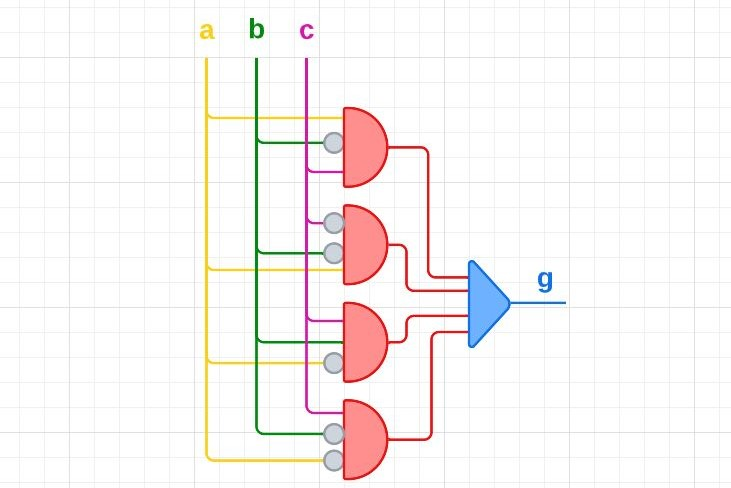
\includegraphics[width= 6cm]{images/cir_sop_fcan.JPG}

        \caption{Circuiti SOP in forma normale e canonica}\label{fig:cir_sop_fnor/can}
    \end{figure}
\end{example}

\newpage
\begin{example}[POS]
    Normale POS: $(\overline{a}+b+c)(a+\overline{b})$\\La trasformo in canonica POS: $(\overline{a}+b+c)(a+\overline{b}+c\overline{c})$\\
    $(\overline{a}+b+c)(a+\overline{b}+c)(a+\overline{b}+\overline{c})$
    
    Inserisco i valori ottenuti all'interno della tabella di verità.
    
    \begin{figure}[!htbp]
        \centering
        \hfill
        \begin{minipage}[b]{.3\columnwidth}
            \centering
            \begin{tabular}{c|c}
                 $a,b,c$ & $h$\\\hline
                 000 & 1\\
                 001 & 1\\
                 010 & 0\\
                 011 & 0\\\hline
                 100 & 0\\
                 101 & 1\\
                 110 & 1\\
                 111 & 1
            \end{tabular}
        \end{minipage}\hfill
        \begin{minipage}[b]{.3\columnwidth}
            \centering
            In POS ragioniamo in maniera duale: identifico quale somma di letterali riulterà 0.
            
            Es. $\overline{a}+b+c$ vale $\overline{a}=1, b=0, c=0$ e inserisco 0 nella tabella in corrispondenza del valore $100$.
        \end{minipage}\hspace*{\fill}
    \end{figure}
    
    Questo perchè vogliamo trovare i valori per cui la somma sia uguale a 0 (ovvero quando tutti i termini valgono 0).
    
    \begin{figure}[!htbp]
        \centering
        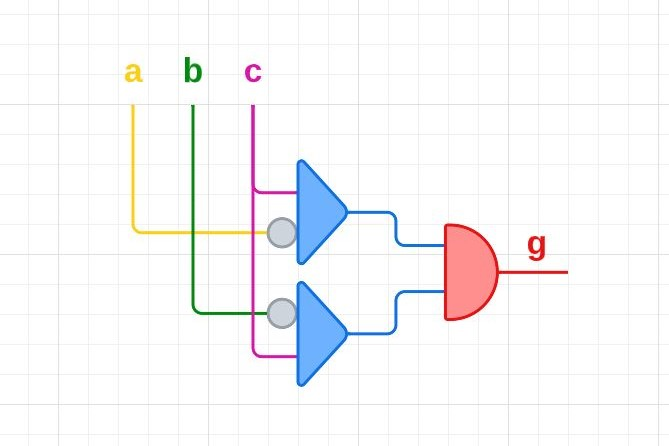
\includegraphics[width= 6cm]{images/cir_pos_fnor.JPG}\hfil
        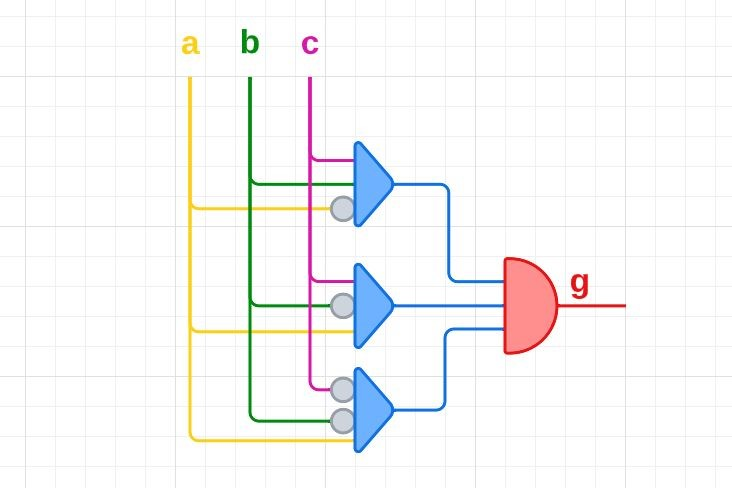
\includegraphics[width= 6cm]{images/cir_pos_fcan.JPG}

        \caption{Circuiti POS in forma normale e canonica}\label{fig:cir_pos_fnor/can}
    \end{figure}

\end{example}

In questo modo, con la tabella di verità, è molto facile passare da SOP a POS e viceversa.
    
La SOP canonica di $h$ sarà data dai valori corrispondenti a 1 nella tabella $h$.
Mentre la POS canonica di $g$ sarà data dai valori corrispondenti a 0 nella tabella $g$.

Infine, l'importanza della SOP e della POS è collegata all'utilità nei circuiti interessati.
La SOP è formata da porte AND che confluiscono in OR. La POS da porte OR che confluiscono in AND.

\subsection{Altri operatori}
Oltre agli operatori fondamentali (AND, OR, NOT) esistono altri operatori che ci permettono di semplificare i nostri circuiti.
\subsubsection*{XOR o OR ESCLUSIVO}
L'operatore XOR vale 1 solo se uno dei due ingressi vale 1, altrimenti 0.

\begin{figure}[htp]
    \centering
    \hfill
    \begin{minipage}[b]{.3\columnwidth}
        \centering
        \begin{tabular}{c|c}
             $a,b$ & $a\oplus b$\\\hline
             00 & 0\\
             01 & 1\\
             10 & 1\\
             11 & 0
        \end{tabular}
        \caption{Tabella di verità dello xor}\label{tab:boole_xor}
    \end{minipage}\hfill
    \begin{minipage}[b]{.3\columnwidth}
        \centering
        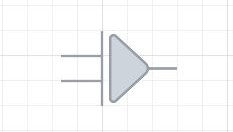
\includegraphics[width = 5cm]{images/xor.JPG}
        \caption{Porta logica dello xor}\label{fig:boole_xor}
    \end{minipage}\hspace*{\fill}
\end{figure}
\begin{center}
\setlength{\tabcolsep}{30pt}
\begin{tabular}{c c}
    Forma canonica SOP & Forma canonica POS\\
    $\overline{a}b+a\overline{b}$ & $(a+b)(\overline{a}+\overline{b})$
\end{tabular}
\end{center}

\mycomment{ % Argomento non trattato
\subsubsection*{XNOR o XOR NEGATO}
L'operatore XNOR è il complementare dello XOR, vale 1 solo quando i due ingressi valgono entrame o 1 o 0.

\begin{figure}[htp]
    \centering
    \hfill
    \begin{minipage}[b]{.3\columnwidth}
        \centering
        \begin{tabular}{c|c}
             $a,b$ & $\overline{a\oplus b}$\\\hline
             00 & 0\\
             01 & 1\\
             10 & 1\\
             11 & 0
        \end{tabular}
        \caption{Tabella di verità dello xnor}\label{tab:boole_xnor}
    \end{minipage}\hfill
    \begin{minipage}[b]{.3\columnwidth}
        \centering
        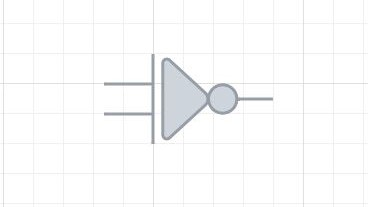
\includegraphics[width = 5cm]{images/xnor.JPG}
        \caption{Porta logica dello xnor}\label{fig:boole_xnor}
    \end{minipage}\hspace*{\fill}
\end{figure}
\begin{center}
\setlength{\tabcolsep}{30pt}
\begin{tabular}{c c}
    Forma canonica SOP & Forma canonica POS\\
    $ab+\overline{a}\overline{b}$ & $(\overline{a}+b)(a+\overline{b})$
\end{tabular}
\end{center}


\begin{question}[Lo XOR è associativo?]
    La risposta è si, ma vediamo il perchè:
    \begin{center}
    $(a\oplus b)\oplus c=^?a\oplus (b\oplus c)$\\
    $(\overline{a}b+\overline{b}a)\oplus c=$\\
    $(\overline{\overline{a}b+a\overline{b}})c+(\overline{a}b+a\overline{b})\overline{c}=$\\
    $\overline{a}\overline{b}c+abc+\overline{a}b\overline{c}+a\overline{b}\overline{c}=$\\Raccolgo $\overline{a}$: 
    $\overline{a}(\overline{b}c+b\overline{c})+a(bc+\overline{b}\overline{c})=$\\Applico lo XOR tra b e c: 
    $\overline{a}(b\oplus c)+a(\overline{b\oplus c})=a\oplus(b\oplus c)$\\E' uno XOR tra $a$ e $b\oplus c$ che mi garantisce il risultato atteso.
    \end{center}
\end{question}
}

\subsubsection*{NAND}
La NAND (NOT-AND) è la complementare della AND e vale 1 solo se il risultato del prodotto degli ingressi è uguale a 0.

\begin{figure}[htp]
    \centering
    \hfill
    \begin{minipage}[b]{.3\columnwidth}
        \centering
        \begin{tabular}{c|c}
             $a,b$ & $\overline{ab}$\\\hline
             00 & 1\\
             01 & 1\\
             10 & 1\\
             11 & 0
        \end{tabular}
        \caption{Tabella di verità della NAND}\label{tab:boole_nand}
    \end{minipage}\hfill
    \begin{minipage}[b]{.3\columnwidth}
        \centering
        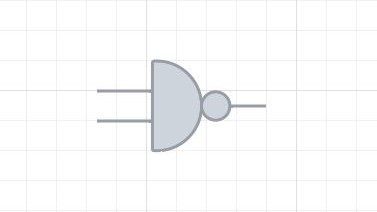
\includegraphics[width = 5cm]{images/nand.JPG}
        \caption{Porta logica della NAND}\label{fig:boole_nand}
    \end{minipage}\hspace*{\fill}
\end{figure}

Come vedremo successivamente è possibile creare formule SOP e POS con sole NAND.

\begin{center}
\setlength{\tabcolsep}{28pt}
\begin{tabular}{m{5cm} m{5cm}}
    SOP con sole NAND & POS con sole NAND\\
    E' conveniente perchè si mantiene il sistema di un'operazione SOP ma utilizzando sempre la stessa porta. A livello realizzativo è più semplice per il calcolatore. & Non è conveniente perchè aumenta solo il numero di operatori utilizzati.
\end{tabular}
\end{center}
Operazioni con il NAND:
\begin{center}
    $\overline{a}=\overline{aa}$\\$ab=\overline{\overline{ab}}=\overline{\overline{ab}\overline{ab}}$\\$a+b=\overline{\overline{a}\overline{b}}=\overline{\overline{aa}\overline{bb}}$
\end{center}

\subsubsection*{NOR}
Il NOR (NOT-OR) `e il complementare dell'OR e vale 1 solo se il risultato della somma degli ingressi è uguale a 0.

\begin{figure}[htp]
    \centering
    \hfill
    \begin{minipage}[b]{.3\columnwidth}
        \centering
        \begin{tabular}{c|c}
             $a,b$ & $\overline{a+b}$\\\hline
             00 & 1\\
             01 & 0\\
             10 & 0\\
             11 & 0
        \end{tabular}
        \caption{Tabella di verità del NOR}\label{tab:boole_nor}
    \end{minipage}\hfill
    \begin{minipage}[b]{.3\columnwidth}
        \centering
        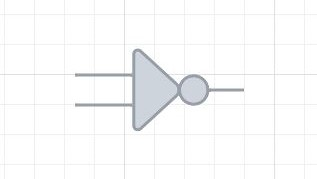
\includegraphics[width = 5cm]{images/nor.JPG}
        \caption{Porta logica del NOR}\label{fig:boole_nor}
    \end{minipage}\hspace*{\fill}
\end{figure}

Anche in questo caso è possibile creare formule SOP e POS con soli NOR.

\begin{center}
\setlength{\tabcolsep}{28pt}
\begin{tabular}{m{5cm} m{5cm}}
    SOP con sole NOR & POS con sole NOR\\
    Non è conveniente perchè aumenta solo il numero di operatori utilizzati. & E' conveniente perchè si mantiene il sistema di un'operazione POS ma utilizzando sempre la stessa porta.
\end{tabular}
\end{center}
Operazioni con il NOR:
\begin{center}
    $\overline{a}=\overline{a+a}$\\$ab=\overline{\overline{a}+\overline{b}}=\overline{\overline{a+a}+\overline{b+b}}$\\$a+b=\overline{\overline{a+b}}=\overline{\overline{a+b}+\overline{a+b}}$
\end{center}

\begin{osservation}[Se ho più di due ingressi cosa succede?]
    Il risultato è lo stesso della forma normale ma il procedimento per raggiungerlo cambia. Perchè con il NAND e NOR si hanno più complementazioni che vengono semplificate.
\end{osservation}

Per approfondire vedi Esercizio \ref{es:nand_nor}.

Ora risulta più chiara l'importanza delle porte NAND e NOR: queste porte possiedono la proprietà di completezza funzionale. 
Vuol dire che ogni altra funzione logica (AND, OR, NOT, etc.) può essere implementata utilizzando solamente porte NAND nella SOP, NOR nella POS, diventando così le uniche due porte logiche universali.


\subsection{Minimizzazione}
Quando possiamo definire che una rete è minimale?

Una rete AND-TO-OR/OR-TO-AND è minimale se:
\begin{itemize}
    \item tra tutte le reti che realizzano la funzione data, la rete ha il minimo numero di porte AND/OR;
    \item tra tutte le reti con numero minimo di porte, la rete ha il minimo numero di ingressi per ogni porta.
\end{itemize}
\begin{osservation}
    Potranno esistere più versioni minimali di una rete.
\end{osservation}
Detto ciò, un'espressione SOP/POS è minimale se:
\begin{itemize}
    \item tra tutte le espressioni SOP/POS che realizzano la funzione $f$, l'espressione ha il minimo numero di termini prodotto/somma;
    \item tra tutte le espressioni SOP/POS che realizzano i termini $f$, l'espressione ha il minimo numero di letterali per ogni termine.
\end{itemize}
Esistono vaire tecniche per effetture la minimizzazione. Quella che useremo sarà utilizzabile con massimo 4 variabili.

\subsubsection*{Tecnica delle mappe di Karnaugh (K-Mappe)}
La tecnica delle mappe di Karnaugh permette di individuare i termini prodotto/somma adiacenti. Ovvero quando differiscono solo di una variabile (vera e complementata).
\begin{example}
    $a\overline{b}c+a\overline{b}\overline{c}$
    
    Notiamo che possiamo raccogliere $a\overline{b}$ essendo in comune in tutti e due i termini. Avremo quindi $a\overline{b}(c+\overline{c})$ che darà come risultato $a\overline{b}$.
\end{example}

Una \textbf{K-mappa} è una visualizzazione della tavola di verità come tabella a due ingressi. Le K-mappe si ottengono stendendo la tavola di verità per trovare i termini che differiscono per una variabile.
Capiamo meglio con gli esempi che seguono:

\begin{example}
\begin{equation}\label{ex:eq:mdk}
    \overline{a}\overline{b}c+a\overline{b}c+a\overline{b}\overline{c}+abc
\end{equation}
    
    
    Stendiamo la tavola di verità dell'equazione:
    \begin{table}[ht]
        \centering
        \begin{tabular}{c|c}
            $abc$ & $f$ \\\hline
            000 & 0\\
            001 & 1\\
            010 & 0\\
            011 & 0\\\hline
            100 & 1\\
            101 & 1\\
            110 & 0\\
            111 & 1
            
        \end{tabular}
        \caption{Tavola di verità dell'equazione \ref{ex:eq:mdk}}
        \label{tab:ex:eq:tdv}
    \end{table}

La K-mappa, a questo punto, si realizzerà con le colonne che fanno riferimento ai valori di $a$, mentre le righe a quelli di $b$ e $c$.
La tabella sarà quindi una matrice che conterrà i termni e valori della tabella di verità con l'unica differenza che le coppie $bc$ saranno scritte come $00,01,11,10$ perchè le righe devono essere adiacenti (devono differire solo di uno 0 o 1).

\begin{table}[ht]
    \centering
    \begin{tabular}{|c||c|c|}
        \hline \diagbox[width=1cm]{\textbf{bc}}{\textbf{a}} & \textbf{0} & \textbf{1}\\\hline\hline
        \textbf{00} & 0 & \textbf{1} \\\hline
        \textbf{01} & \textbf{1} & \textbf{1} \\\hline
        \textbf{11} & 0 & \textbf{1} \\\hline
        \textbf{10} & 0 & 0 \\\hline
    \end{tabular}
    \caption{K-mappa dell'espressione \ref{ex:eq:mdk}}
    \label{tab:ex:eq:mkd}
\end{table}

Ora per scrivere l'espressione raccolgo a due a due i mintermini adiacenti ($es. 100,101$). In questo modo mi trovo i valori che differiscono solo di una variabile. Il secondo passaggio è quello di scrivere l'espressione, guardando cosa hanno in comune i mintermini considerati secondo i valori di $ab$ e $cd$ nella tabella. Si scriverà quindi il letterale normale se in tabella corrisponde a 1, complementato se corrisponde a 0 ($es. 001,101=\overline{b}c$ oppure $es. 101,111=ac$). Come ultima cosa aggiungiamo i termini che non si trovano in adiacenza con nessun'altro termine.
In questo modo il risultato sarà minimizzato.

\textbf{SOP minimale:} $a\overline{b}+\overline{b}c+ac$
\end{example}

\begin{example}
    Cosa accade con 4 variabili?
    \begin{table}[ht]
        \centering
        \begin{tabular}{c|c}
        $abcd$ & $f$ \\\hline
        0000 & 0\\
        0001 & 0\\
        0010 & 0\\
        0011 & 1\\\hline
        0100 & 1\\
        0101 & 1\\
        0110 & 0\\
        0111 & 0\\\hline
        1000 & 0\\
        1001 & 1\\
        1010 & 0\\
        1011 & 1\\\hline
        1100 & 1\\
        1101 & 1\\
        1110 & 0\\
        1111 & 1
    \end{tabular}
        \caption{Tavola di verità}
        %\label{tab:my_label}
    \end{table}
    
    Con 4 variabili si aggiunge alla coppia $cd$ la coppia $ab$.
    \begin{table}[ht]
    \centering
    \begin{tabular}{|c||c|c|c|c|}
        \hline \diagbox[width=1cm]{\textbf{ab}}{\textbf{cd}} & \textbf{00} & \textbf{01} & \textbf{11} & \textbf{10} \\\hline\hline
        \textbf{00} & 0 & 0 & \textbf{1} & 0 \\\hline
        \textbf{01} & \textbf{1} & \textbf{1} & 0 & 0 \\\hline
        \textbf{11} & \textbf{1} & \textbf{1} & \textbf{1} & 0 \\\hline
        \textbf{10} & 0 & \textbf{1} & \textbf{1} & 0 \\\hline
    \end{tabular}
    \caption{K-mappa}
    \label{tab:ex:eq:mkqm}
\end{table}

Rispetto all'esempio precendente cambia la grandezza della mappa (vedi Tabella \ref{tab:ex:eq:mkqm}). Per tanto come prima cosa dobbiamo trovare gli 1 nel cubo massiamale. Questo vuol dire trovare 4 1 adiacenti disposti a quadrato o lungo una riga/colonna, per identificane le variabili comuni. Successivamente copriremo i casi degli 1 in doppio e infine i singoli 1 non adiacenti a nessun'altro 1.
In questo modo possiamo trovare la SOP minimale.

\textbf{SOP minimale:} $ad+b\overline{c}+\overline{b}cd$

Per trovare la POS invece dobbiamo attuare lo stesso procedimento ma raccogliendo gli 0 e scrivendo la variabile in forma normale se vale 0, altrimenti complementata.

\textbf{POS minimale:} $(b+d)(\overline{c}+d)(a+b+c)(a+\overline{b}+\overline{c})$

\begin{description}
    \item[N.B.] I quadrati e le coppie valgono anche per gli angoli della tabella o passando dalla prima riga/colonna all'ultima.
\end{description}
\end{example}


\subsection*{Tavole con valori indeterminati}
Nelle tavole di verità possono esserci dei valori indeterminati chiamati \textit{don't care}, rappresentati con $\delta$ o -.
La presenza di questi valori è giustificata da due motivi:
\begin{enumerate}
    \item non si possono rappresentare gli ingressi ($\bullet$);
    \item non si possono rappresentare le uscite (\textbf{x}).
\end{enumerate}

\begin{example}
    Dato $x$ come valore compreso tra $[0;5]$, stendere la tavola di verità che rappresenta $y$ compreso tra $[0;5]$.
    
    \begin{table}[ht]
        \centering
        \begin{tabular}{c|c}
             $x_2 x_1 x_0$ & $y_2 y_1 y_0$\\\hline
             000 & 010\\
             001 & 011\\
             010 & 100\\
             011 & 101\\\hline
             100 & 011\\
             101 & 100\\
             110 & - -\\
             111 & - -
        \end{tabular}
        \caption{Tavola di verità con più output}
        %\label{tab:my_label}
    \end{table}
    Per trovare i minimali stendiamo le mappe di Karnaugh.
    
    \begin{table}[ht]
    \centering
        \begin{tabular}{|c||c|c|c|c|}
            \hline \diagbox[width=1.5cm]{\textbf{$x_2$}}{\textbf{$x_1 x_0$}} & \textbf{00} & \textbf{01} & \textbf{11} & \textbf{10}\\\hline\hline
            \textbf{0} & 0 & 0 & 1 & 1\\\hline
            \textbf{1} & 0 & 1 & - & -\\\hline
        \end{tabular}
        \caption{Mappa per output $y_2$}
        %\label{tab:ex:eq:mkd}
    \end{table}
    
    I - possono assumere il valore di cui ho bisogno, nella maniera più conveniente che mi permette di avere il cubo di valori più grande. In questo caso considero i don't care come 1.
    
    \textbf{SOP minimale:} $x_1+x_2x_0$
    
    \textbf{POS minimale:} $(x_2+x_1)(x_1+x_0)$
    
    Applico le stesse regole alle ultime due uscite $y_1$ e $y_0$.
    \begin{table}[ht]
    \centering
        \begin{tabular}{|c||c|c|c|c|}
            \hline \diagbox[width=1.5cm]{\textbf{$x_2$}}{\textbf{$x_1 x_0$}} & \textbf{00} & \textbf{01} & \textbf{11} & \textbf{10}\\\hline\hline
            \textbf{0} & 1 & 1 & 0 & 0\\\hline
            \textbf{1} & 1 & 0 & - & -\\\hline
        \end{tabular}
        \caption{Mappa per output $y_1$}
        %\label{tab:ex:eq:mkd}
    \end{table}
    
    \textbf{SOP minimale:} $\overline{x_2}\overline{x_1}+\overline{x_1}\overline{x_0}$
    
    \textbf{POS minimale:} $\overline{x_1}(\overline{x_2}+\overline{x_0})$
    
    \begin{table}[ht]
    \centering
        \begin{tabular}{|c||c|c|c|c|}
            \hline \diagbox[width=1.5cm]{\textbf{$x_2$}}{\textbf{$x_1 x_0$}} & \textbf{00} & \textbf{01} & \textbf{11} & \textbf{10}\\\hline\hline
            \textbf{0} & 0 & 1 & 1 & 0\\\hline
            \textbf{1} & 1 & 0 & - & -\\\hline
        \end{tabular}
        \caption{Mappa per output $y_0$}
        %\label{tab:ex:eq:mkd}
    \end{table}
    
    \textbf{SOP minimale:} $\overline{x_2}x_0+x_2\overline{x_0}$
    
    \textbf{POS minimale:} $(x_2+x_0)(\overline{x_2+\overline{x_0}})$
    
    Infine per rappresentare la rete corrispondente posso sceglere le forme minimali più convenienti in termini di operatori utilizzati.
    
\end{example}


\section{Reti combinatorie}
Analizziamo ora le porte logiche (accennate nella sezione \ref{sec:algebra_di_boole}) più nel dettaglio.

Sono reti combinatorie:
\begin{itemize}
    \item I terminali di ingresso;
    \item $\overline{N}$ se $N$ è una rete combinatoria;
    \item $N_1*N_2$ se $N_1$ e $N_2$ sono reti combinatorie;
    \item $N_1+N_2$ se $N_1$ e $N_2$ sono reti combinatorie;
    \item Sono reti combinatorie tutte e sole le reti descritte sopra.
\end{itemize}

\begin{description}
    \item[N.B.] Con le reti combinatorie si possono formare anche dei cicli.
\end{description}


Stando a quanto detto finora, ad ogni espressione booleana corrisponde una rete combinatoria.
\begin{example}
    $(x_1+\overline{x_2}+x_3)x_1x_2\overline{x_3}$
    \begin{figure}[ht]
        \centering
        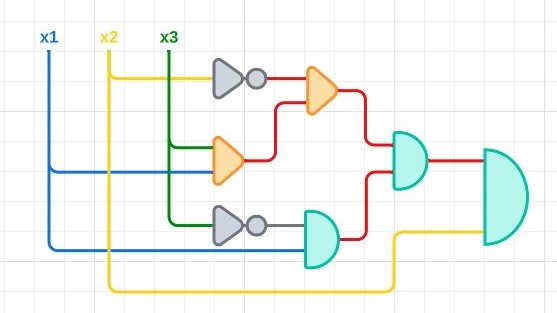
\includegraphics[width=9cm]{images/reti_combinatorie.JPG}
        \caption{Esempio di rete combinatoria}
        \label{fig:es:reti_combinatorie}
    \end{figure}
\end{example}

\subsection*{Procedimento di sintesi di una rete combinatoria}
Per sintetizzare una rete combinatoria partendo da un dato problema, i passi da seguire sono i seguenti:
\begin{itemize}
    \item Leggere la specifica verbale o traccia del problema;
    \item Ricavare l'espressione booleana (se necessario);
    \item Stendere la tavola di verità;
    \item Trovare le espressioni minimali con le K-Mappe;
    \item Disegnare la rete combinatioria;
    \item Analizzare (se richiesto).
\end{itemize}
Per approfondire vedi Esercizio \ref{ex:innaffio}.

\subsection*{Analisi di una rete combinatoria}
Il procedimento opposto di quanto descritto sopra è formato dai seguenti passi:
\begin{itemize}
    \item Partire dalla rete combinatoria data;
    \item Ricavare le espressioni booleane;
    \item Stendere la tavola di verità;
    \item Semplificare le espressioni (se necessario);
    \item Scrivere una descrizione verbale.
\end{itemize}

\newpage
\section{Esercizi svolti}
\begin{exercise}[Costruire una funzione di maggioranza che vale 1 se almeno la metà delle variabili vale 1]\label{es:nand_nor}

Per costruire la funzione di maggioranza come prima cosa la rappresentiamo su un tabella di verità e identifichiamo con $m_i$ i mintermini e con $M_i$ i maxtermini.
\begin{table}[ht]
    \centering
    \begin{tabular}{|c||c|c|}
         \hline & $a,b,c$ & $f$\\\hline\hline
         $M_0$ & 000 & 0\\\hline
         $M_1$& 001 & 0\\\hline
         $M_2$& 010 & 0\\\hline
         $m_3$& 011 & 1\\\hline
         $M_4$& 100 & 0\\\hline
         $m_5$& 101 & 1\\\hline
         $m_6$& 110 & 1\\\hline
         $m_7$& 111 & 1\\\hline
    \end{tabular}
    \caption{Tabella di verità della funzione di maggioranza}
    \label{tab:verit_fmagg}
\end{table}

Otteniamo ora le forme SOP e POS:

\textbf{SOP:} $m_3+m_5+m_6+m_7 = \overline{a}bc+a\overline{b}c+ab\overline{c}+abc$

\textbf{POS:} $M_0+M_1+M_2+M_4 = (a+b+c)(a+b+\overline{c})(a+\overline{b}+c)(\overline{a}+b+c)$

Se vogliamo rappresentare la funzione con sole NAND o soli NOR, moltiplichiamo il termine $abc$ nella SOP e $a+b+c$ nella POS, tante volte quanti sono i termini che vogliamo semplificare.

\textbf{SOP:} $bc+ac+ab$

\textbf{POS:} $(a+b)(a+c)(b+c)$

Rappresentiamo ora i nostri risultati in ALL-NAND e ALL-NOR.

\textbf{ALL-NAND: } Partiamo dalla SOP e sostituiamo ogni operatore con una NAND.\\$f=\overline{\overline{bc}\overline{ac}\overline{ab}}$.

\textbf{ALL-NOR: } Partiamo dalla POS e sostituiamo ogni operatore con una NOR.\\$f=\overline{\overline{a+b}+\overline{a+c}+\overline{b+c}}$.

\begin{figure}[!htbp]
        \centering
        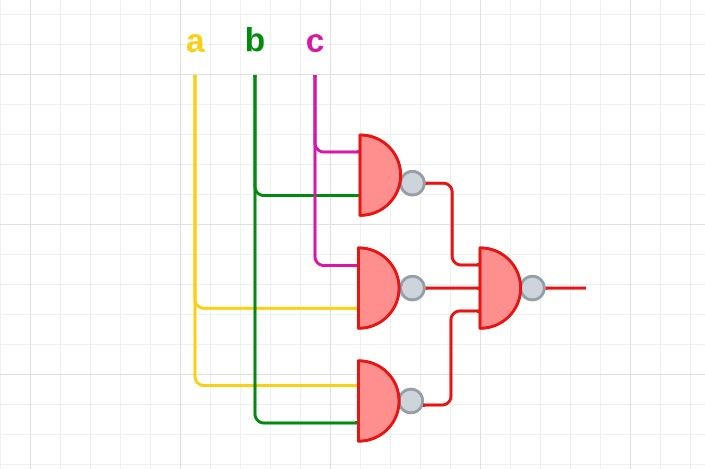
\includegraphics[width = 6cm]{images/es_nand.JPG}\hfil
        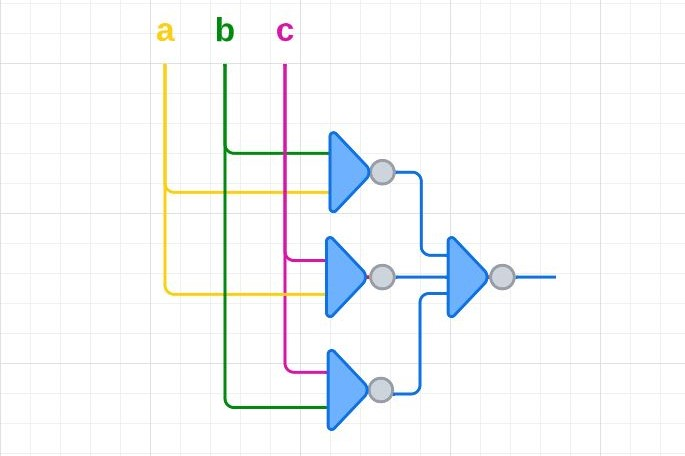
\includegraphics[width = 6cm]{images/es_nor.JPG}

        \caption{Circuiti in ALL-NAND e ALL-NOR}\label{es:fig:cir_all_nand/nor}
    \end{figure}
\end{exercise}

\begin{exercise}
    Data la funzione $f=(\overline{a}b\overline{c})(bc+\overline{a}c)$ trovare la normale e canonica SOP e POS, tracciare la tabella di verità. Infine inserire nella tabella le funzioni $\Tilde{f}$(duale di f) e $\overline{f}$(complementare di f).
    
    Applichiamo de Morgan sulla funzione $(\overline{a}(\overline{b}+\overline{c}))(bc+\overline{a}c)$. Applichiamo ora la proprietà distributiva $(\overline{a}\overline{b}+\overline{a}\overline{c})(bc+\overline{a}b)$, svolgiamo le moltiplcazioni $\overline{a}\overline{b}bc+\overline{a}\overline{b}\overline{a}b$. Semplificando i termini opposti otteniamo $\overline{a}c+\overline{a}$ e infine per semplificare il primo termine moltiplichiamo per $b\overline{c}$.
    
    In questo modo otteniamo le forme normali SOP e POS (in questo caso sono le stesse): $\overline{a}b\overline{c}$.
    
    Per calcolare le forme canoniche proseguiamo nel seguente modo:
    
    \textbf{Canonica SOP:} l'espressione è già in forma canonica SOP.
    
    \textbf{Canonica POS:} $(\overline{a}+b\overline{b}+c\overline{c})+(a\overline{a}+b+c\overline{c})(a\overline{a}+b\overline{b}+\overline{c})$.
    Trovo ora tutte le combinazioni per $\overline{a}$ fisso, $b$ fisso e $\overline{c}$ fisso.
    \begin{itemize}
        \item[$\overline{a}$:] $(\overline{a}+b+c)(\overline{a}\overline{b}+c)(\overline{a}+b+\overline{c})(\overline{a}+\overline{b}+\overline{c})$
        \item[$b$:] $(a+b+c)(a+b+\overline{c})(\overline{a}+b+c)(\overline{a}+b+\overline{c})$
        \item[$\overline{c}$:] $(a+b+\overline{c})(a+\overline{b}+\overline{c})(\overline{a}+b+\overline{c})(\overline{a}+\overline{b}+c)$
    \end{itemize}
    
    Dopo aver eliminato i termini ripetuti, reppresentiamo i valori ottenuti nella tabella di verità.
    \begin{table}[ht]
        \centering
        \begin{tabular}{|c|c|c|c|}
             \hline$abc$ & $f$ & $\Tilde{f}$ & $\overline{f}$ \\\hline\hline
             000 & 0 & 1 & 1\\
             001 & 0 & 1 & 1\\
             010 & 1 & 1 & 0\\
             011 & 0 & 1 & 1\\\hline
             100 & 0 & 1 & 1\\
             101 & 0 & 0 & 1\\
             110 & 0 & 1 & 1\\
             111 & 0 & 1 & 1\\\hline
        \end{tabular}
        \caption{Tavola di verità}
        %\label{tab:my_label}
    \end{table}
    
    \textbf{Duale:} $\overline{a}+b+\overline{c}$. Essendo POS, per la duale trovo i valori di 0 per cui è verificata (solo per 101).
\end{exercise}


\begin{exercise}\label{ex:innaffio}
    Progettare un circuito che regola l'accensione di un'impianto di innaffiamento. L'impianto si attiva se si verificano \textbf{uno} dei tre eventi:
\begin{itemize}
    \item Il sensore crepuscolare rileva che la luce è sotto una certa soglia;
    \item Il timer è impostato sull'ora di accensione e non piove;
    \item Non è l'ora di accensione ma la temperatura è sopra una certa soglia.
\end{itemize}
Come prima cosa dobbiamo definire le variabili di ingresso per la nostra funzione.

\textbf{Ingresso:}
$$
\text{Sensore }A=
\begin{cases}
1 \text{ luce sotto la soglia}\\
0 \text{ altrimenti}
\end{cases}
$$
$$
\text{Ora }O=
\begin{cases}
1 \text{ se è giusta}\\
0 \text{ altrimenti}
\end{cases}
$$
$$
\text{Piove }P=
\begin{cases}
1 \text{ se piove}\\
0 \text{ altrimenti}
\end{cases}
$$
$$
\text{Temperatura }T=
\begin{cases}
1 \text{ se temperatura } > \text{ della soglia}\\
0 \text{ altrimenti}
\end{cases}
$$

\textbf{Uscita:}
$$
\text{Innaffiamento }INN=
\begin{cases}
1 \text{ acceso}\\
0 \text{ spento}
\end{cases}
$$

Ricavaimo ora la nostra espressione:
\begin{equation}\label{eq:innaff}
    A+O\overline{P}+\overline{O}T
\end{equation}

Stendiamo la tavola di verità.
\begin{table}[ht]
    \centering
    \begin{tabular}{c|c}
         $AOPT$ & $f$\\\hline
         0000 & 0\\
         0001 & 1\\
         0010 & 0\\
         0011 & 1\\\hline
         0100 & 1\\
         0101 & 1\\
         0110 & 0\\
         0111 & 0\\\hline
         1000 & 1\\
         1001 & 1\\
         1010 & 1\\
         1011 & 1\\\hline
         1100 & 1\\
         1101 & 1\\
         1110 & 1\\
         1111 & 1\\
    \end{tabular}
    \caption{Tavola di verità}
    %\label{tab:aotp}
\end{table}

Per verificare se l'espressione \ref{eq:innaff} è la migliore utilizziamo le K-Mappe.

Da qui possiamo ricavare le espressioni minimali SOP e POS.

\textbf{SOP minimale:} $A+O\overline{P}+\overline{O}T$

\textbf{POS minimale:} $(A+\overline{O}+\overline{P})(A+O+T)$

\end{exercise}